\documentclass[10pt, english, singlespacing, liststotoc, toctotoc, headsepline, chapterinoneline]{ClassThesis} % The class file specifying the document structure

\usepackage[utf8]{inputenc} % Required for inputting international characters
\usepackage[T1]{fontenc} % Output font encoding for international characters

%\usepackage{mathpazo} % Use the Palatino font by default
\usepackage{mathptmx}
%\usepackage{stix} % tipo de fuente
\usepackage{microtype} 
\usepackage{datetime}
\usepackage{comment}

\usepackage{mathtools} % símbolos extensibles (contiene amsmath)
\usepackage{amssymb} % símbolos matemáticos
\usepackage{amsthm} % para teoremas, lemas, ...
\usepackage{mathrsfs} % para usar \mathscr{}
\usepackage{tensor} % índices en cualquier lado
\usepackage{cancel} % tachar
\usepackage{dsfont} % usar fuente bbm en modo mates (para poner la identidad en vd)

\usepackage{array} % arrays
\usepackage{multirow} % redimensionar, unir celdas, ...
\usepackage{blkarray} % arrays en bloques
\usepackage{footnote} % notas a pie de pagina
\usepackage{multicol}

\usepackage{float} % para figuras (las fija, [H], ...)
\usepackage{chngcntr}
\counterwithout{figure}{chapter}

\renewcommand{\theenumi}{\roman{enumi}}
\renewcommand{\thefigure}{\Roman{figure}} 
\renewcommand{\thesubfigure}{\Alph{subfigure}}
\newcommand\diagram[2]{\schema{\schemabox{#1}}{\schemabox{#2}}}
\newtheorem{theorem}{Teorema}[section]
\newtheorem{example}{Ejemplo}[section]
\newtheorem{lemma}{Lema}
\newtheorem{definition}{Definición}[section]
\newtheorem{comentario}{Comentario}[section]
\def\proof{\paragraph{Demostraci\'on:\\}}
\def\endproof{\hfill$\blacksquare$}
\DeclareMathOperator*{\argmax}{arg\,max}


% chktex-file 12
% chktex-file 13
% chktex-file 44

\usepackage[backend=bibtex, style=authoryear, natbib=true, maxcitenames=2, maxbibnames=20, minbibnames=1]{biblatex} % Use the bibtex backend with the authoryear citation style (which resembles APA) % sorting=none for citation order

\addbibresource{references.bib} % The filename of the bibliography
\setlength\bibitemsep{1.5\itemsep}

\usepackage[autostyle=true]{csquotes} % Required to generate language-dependent quotes in the bibliography
\usepackage{listings}
\lstdefinestyle{terminal}{
  backgroundcolor=\color{white},   % Fondo blanco
  basicstyle=\color{black}\ttfamily, % Texto negro en fuente monoespaciada
  keywordstyle=\color{blue}\bfseries, % Palabras clave en azul y negrita
  commentstyle=\color{green!70}\ttfamily, % Comentarios en verde
  stringstyle=\color{red}\ttfamily, % Cadenas en rojo
  morekeywords={sudo, apt-get, install, cd, ls, mkdir, rm, rmdir, cp, mv, echo, cat, nano, vim, grep, find, chmod, chown, systemctl, service, update, upgrade, reboot, shutdown, exit}, % Comandos comunes de terminal
  breaklines=true, % Permitir saltos de línea
  frame=single, % Marco alrededor del código
  framerule=0.5pt, % Grosor del marco
  rulecolor=\color{gray}, % Color del marco
  xleftmargin=0.05\textwidth, % Margen izquierdo
  xrightmargin=0.05\textwidth, % Margen derecho
  aboveskip=1em, % Espacio antes del bloque de código
  belowskip=1em % Espacio después del bloque de código
}
%----------------------------------------------------------------------------------------
%	MARGIN SETTINGS
%----------------------------------------------------------------------------------------

\geometry{
	paper=a4paper, % Change to letterpaper for US letter
	inner=2.5cm, % Inner margin
	outer=3.8cm, % Outer margin
	bindingoffset=.5cm, % Binding offset
	top=1.5cm, % Top margin
	bottom=1.5cm, % Bottom margin
	%showframe, % Uncomment to show how the type block is set on the page
}

%----------------------------------------------------------------------------------------
%	THESIS INFORMATION
%----------------------------------------------------------------------------------------

\thesistitle{Técnologías de computación \\ para datos masivos} % \ttitle
\supervisor{Tomás Fernández Pena} % \supname
\examiner{} % \examname
\degree{Master en Tecnoloxías de Análise \\ de Datos Masivos: Big Data} % \degreename
\author{Luis Ardévol Mesa} % \authorname
\addresses{} % \addressname

\subject{} % Subject area, print it elsewhere with \subjectname
\keywords{} %\keywordnames
\university{Universidad de Santiago de Compostela} % \univname
\department{} % \deptname
\group{} % \groupname
\faculty{Escola Técnica Superior de Enxeñaría} % \facname

\AtBeginDocument{
\hypersetup{pdftitle=\ttitle} % Set the PDF's title to your title
\hypersetup{pdfauthor=\authorname} % Set the PDF's author to your name
\hypersetup{pdfkeywords=\keywordnames} % Set the PDF's keywords to your keywords
}

\begin{document}

\frontmatter % Use roman page numbering style (i, ii, iii, iv...) for the pre-content pages

\pagestyle{plain} % Default to the plain heading style until the thesis style is called for the body content

%----------------------------------------------------------------------------------------
%	TITLE PAGE
%----------------------------------------------------------------------------------------

\begin{titlepage}
\begin{center}

\vspace*{.06\textheight}
{\scshape\LARGE \textcolor{mdtRed}{\univname}\par}\vspace{1.5cm} 
\textsc{}\\[0.5cm] 

\HRule{} \\[0.4cm]
{\huge \bfseries \ttitle\par}\vspace{0.4cm} 
\HRule{} \\[1.5cm] 
 
\begin{minipage}[t]{0.4\textwidth}
\begin{flushleft} \large
\emph{Autor:}\\
\textcolor{mdtRed}{\authorname} 
\end{flushleft}
\end{minipage}
\begin{minipage}[t]{0.4\textwidth}
\begin{flushright} \large
\emph{Profesor:} \\
\textcolor{mdtRed}{\supname} 
\end{flushright}
\end{minipage}\\[3cm]
 
\vfill

\large \textit{\facname\\ \degreename}\\[0.8cm] 
 
\vfill

{\large \today}\\[4cm] % Date
%\includegraphics{Logo} 
 
\vfill
\end{center}
\end{titlepage}


\newgeometry{
	inner=2.5cm, % Inner margin
	outer=3cm, % Outer margin
	bindingoffset=.5cm, % Binding offset
	top=3cm, % Top margin
	bottom=3cm, % Bottom margin
	%showframe, % Uncomment to show how the type block is set on the page
}

%----------------------------------------------------------------------------------------
%	LIST OF CONTENTS/FIGURES/TABLES PAGES
%----------------------------------------------------------------------------------------

\tableofcontents % Prints the main table of contents

%----------------------------------------------------------------------------------------
%	THESIS CONTENT - CHAPTERS
%----------------------------------------------------------------------------------------

\mainmatter{} % Begin numeric (1,2,3...) page numbering

\pagestyle{thesis} % Return the page headers back to the "thesis" style

\chapter{Introducción}\label{Chapter1} 
% chktex-file 8
% chktex-file 12
% chktex-file 13
% chktex-file 44

El avance en la capacidad de generar y almacenar datos ha llevado a la necesidad de transformar los datos crudos en conocimiento accionable que pueda optimizar la toma de decisiones en diversos sectores como salud, seguridad, educación, ciencia y negocios (BI). Para lograrlo, es fundamental desarrollar tecnologías que permitan ver y extraer información útil y conocimiento oculto en los datos, particularmente en grandes cantidades de datos textuales. Gestionar y analizar grandes cantidades de datos textuales puede ayudar a los usuarios a gestionar y hacer uso de este tipo de datos en todo tipo de aplicaciones.

\section{Datos textuales como \textit{Big Data}}
La gestión de texto de lenguaje natural, que abarca desde páginas web y redes sociales hasta literatura científica y documentos gubernamentales, se ha convertido en una prioridad debido a la explosión de datos en temas de todo tipo. Como un tipo especial de \textit{big data}, los datos textuales representan una gran oportunidad para el descubrimiento de conocimiento y optimización de decisiones en múltiples aplicaciones. Un ejemplo de ello son los datos textuales de opiniones (valoraciones de productos, foros, redes sociales, ...). \\

Dado el volumen creciente de datos textuales, es imposible para una persona consumir toda la información relevante en tiempo real, de modo que se requieren sistemas inteligentes de recuperación de información para facilitar el acceso rápido a los datos necesarios. El mundo genera entre 1 y 2 \textit{exabytes} de datos anualmente, de los cuales una gran cantidad es textual. \\

Atendiendo a la estructura de los datos, se pueden clasificar en dos tipos:
\begin{itemize}
\item Los datos estructurados, que cuentan con esquemas bien definidos, son manejados fácilmente por los ordenadores. 
\item Los datos no estructurados, como el texto, necesitan procesamiento computacional para interpretar su contenido, al tener una estructura menos explícita.
\end{itemize}

El procesamiento de lenguaje natural (NLP) aun no ha alcanzado un punto que permita al ordenador entender de forma precisa el texto. Generalmente se usan aproximaciones estadísticas y heurísticas para extraer información y analizar los datos textuales. El texto es de las fuentes de información más útiles ya que 
\begin{itemize}
\item Es la forma más natural de codificar el conocimiento humano. Por ejemplo, el conocimiento científico casi solo existe en literatura científica, los manuales técnicos dan explicaciones detalladas de como operar aparatos, ...
\item Es el tipo de información más frecuente.
\item Es la forma de información más expresiva.
\end{itemize}

\subsection{Recuperación y minería de texto}

\noindent Para gestionar y explotar grandes cantidades de datos textuales, se suele recurrir a dos técnicas. Se aplica la recuperación de textos sobre una gran cantidad de datos textuales para, sobre los datos relevantes extraídos, aplicar minería y obtener conocimiento que usar en distintas aplicaciones.

\subsubsection{Recuperación de texto (\textit{text retrieval})}

No se puede digerir toda la cantidad de información disponible, por lo que son necesarios sistemas inteligentes de recuperación de información para facilitar el acceso rápido a los datos necesarios. Para esto surgen los motores de búsqueda, útiles en cualquier contexto donde haya una gran cantidad de datos textuales, no solo en la \textit{web}. 

\subsubsection{Minería de texto (DM)}

Los datos textuales son ricos en contenido semántico. La minería de texto busca descubrir conocimiento valioso dentro del contenido textual, usando herramientas de \textit{software} inteligentes para descubrir patrones interesantes y opiniones que optimicen la toma de decisiones. El proceso de minería de datos puede describirse como minar los datos textuales para descubrir conocimiento útil. \\

La minería de datos aún no es tan madura como los motores de búsqueda, ya que el texto tiene una estructura menos explícita. El desarrollo de minería inteligente requiere que los ordenadores entiendan el contenido codificado en el texto. 

\subsection{Modos de acceso a la información: Pull vs Push}

En el modo \textit{pull}, el usuario toma la iniciativa de buscar información en el sistema, mientras que este último juega un papel pasivo y espera la petición del usuario. En las consultas, el usuario especifica la información necesaria y el sistema devuelve documentos que considera relevantes. \\

En el modo \textit{push}, el sistema recomienda información anticipando las preferencias y necesidades de información del usuario. Suele funcionar bien cuando el usuario tiene una necesidad de información relativamente estable, como un \textit{hobby}. Aquí, el sistema puede conocer las preferencias e intereses del usuario con adelanto. \\

En la navegación, el usuario se mueve por estructuras que enlazan elementos de información y alcanza información relevante progresivamente. La navegación y las consultas se alternan de forma natural. 

\section{Sistemas de Información Textual (TIS)}

Estos sistemas buscan dar acceso a la información: conectan la información adecuada con el usuario adecuado en el momento adecuado. Ejemplos clásicos son:
\begin{itemize}
\item Motores de búsqueda: permiten al usuario acceder a información textual a través de consultas.
\item Sistemas de recomendación: pueden sugerir información relevante al usuario de forma proactiva. 
\end{itemize}

Se debe realizar un análisis de texto suficiente como para emparejar la información relevante con la información que necesita el usuario. Los elementos de información originales se muestran en su forma original, aunque en ocasiones se muestra a través de resúmenes dinámicos que dependen de la búsqueda del usuario (\textit{snippets}).

\subsection{Análisis del texto}

Un análisis del texto permite adquirir el conocimiento útil codificado en los datos textuales, el cuál no es fácil de obtener sin sintetizar y analizar una gran cantidad de los datos. Por ejemplo, un motor de búsqueda simplemente devuelve las valoraciones relevantes de un producto, mientras que un motor de análisis extrae las opiniones positivas y negativas y compara opiniones de multitud de productos. \\

Los sistemas de información textual anotan una colección de documentos textuales con estructuras (tópicos) relevantes. Estas estructuras añadidas permiten al usuario buscar con restricciones sobre las mismas o navegar siguiéndolas. \\

A diferencia del DM, que se mueve bajo la premisa de descubrir y extraer patrones interesantes en los datos textuales, el NLP se mueve bajo la premisa de entender del texto de lenguaje natural de forma parcial, convertirlo en una forma de representación de conocimiento y hacer inferencia basándose en el conocimiento extraido. 

\subsection{Sistemas de información textual}
Los TIS integran servicios de análisis de contenido basados en procesamiento de lenguaje natural (NLP) para transformar datos textuales crudos en representaciones más significativas, apoyando así la recuperación, categorización y organización de información. Se suele combinar el aprendizaje automático estadístico con conocimiento linguístico limitado. Las técnicas poco profundas son robustas, pero un análisis semántico profundo solo es factible en dominios específicos. \\

Algunas habilidades, como la de resumir documentos, requieren técnicas de NLP más profundas que otras, como una simple búsqueda. Sin embargo, la mayorías de TIS usan técnicas poco profundas, como bolsas de palabras. 

\begin{figure}[h]
\centering
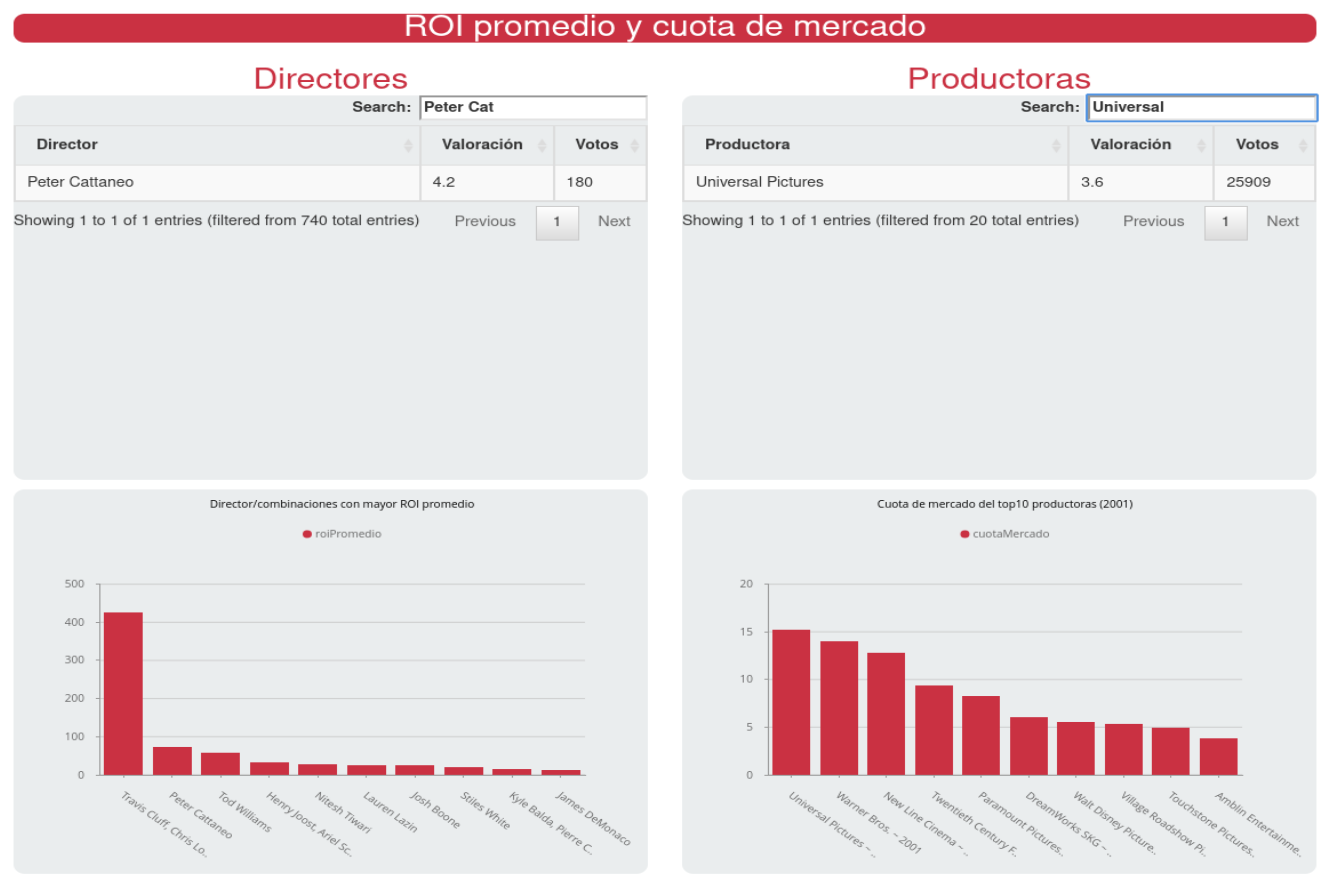
\includegraphics[width=0.5\textwidth]{fotos/1.png}
\caption{Esquema conceptual de un TIS}
\label{fig:1}
\end{figure}

\noindent Existen varias formas de organizar la información en un TIS:

\begin{itemize}
    \item \textbf{Búsqueda}: toma una consulta del usuario y devuelve documentos relevantes.
    \item \textbf{Filtrado y Recomendación}: monitoriza el flujo de datos, selecciona los ítems relevantes para los intereses del usuario y luego recomienda los items relevantes (o filtra los no relevantes). Un sistema de recomendación tiene como objetivo recomendar información relevante al usuario, mientras que un sistema de filtrado tiene como objetivo filtrar la información no relevante, permitiendo que el usuario mantenga solo los \textit{items} relevantes.
    \item \textbf{Categorización}: clasifica un objeto textual en una o varias categorías predefinidas. Puede anotar los objetos con todo tipo de categorías significativas, enriqueciendo la representación de los datos textuales. En este caso hay dos tipos de errores, los falsos positivos y los falsos negativos; hay que ver que métrica de rendimiento se le da al clasificador, dando más o menos \textit{penalty} a un error concreto. Estos sistemas son tradicionales, y se usaban para, por ejemplo, clasificar correos electrónicos como \textit{spam}.
    \item \textbf{Resumen}: toma uno o varios documentos de texto y genera un resumen conciso de los contenidos esenciales. Reduce el esfuerzo humano de digerir grandes cantidades de información textual.
    \item \textbf{Análisis de temáticas}: toma una serie de documentos y extrae y analiza los temas en ellos. Los temas aydan a digerir la información y permiten navegar por el texto de forma cómoda. Se puede combinar con datos no textuales, como tiempo, localización u otros metadatos. De este modo, es capaz de generar patrones de interés (tendencias temporales de temáticas, distribución espacio-temporal del tópicos, etc). Es tecnología no supervisada, por lo que los temas no están predefinidos, los da el propio algoritmo.
    \item \textbf{Extracción de información}: Extrae entidades y relaciones de entidades con otras áreas de conocimiento. 
    \item \textbf{Clustering}: descubre grupos de objetos textuales similares (términos, oraciones, documentos, etc). Ayuda a los usuarios a explorar un espacio de la información, y es útil para descrubrir \textit{outliers}. 
    \item \textbf{Visualización}: permite representar visualmente patrones en los datos textuales.
\end{itemize}
VER LOS PROCESOS DEL MASTER Y DE LOS DEMONIOS 
\chapter{Datos textuales}\label{Chapter2} 
% chktex-file 8
% chktex-file 12
% chktex-file 13
% chktex-file 44

\section{Procesamiento de lenguaje natural}

El procesamiento de lenguaje natural (NLP) se ocupa de desarrollar técnicas computacionales para permitir que una computadora entienda el significado del texto en lenguaje natural. El NLP es una base fundamental de los sistemas de información textual (TIS) porque la efectividad de un TIS en ayudar a los usuarios a acceder y analizar datos textuales depende en gran medida de qué tan bien el sistema pueda entender el contenido de los datos textuales. Por lo tanto, el análisis de contenido es lógicamente el primer paso en el análisis y gestión de datos textuales. \\

Mientras que un humano puede entender instantáneamente una oración en su idioma nativo, resulta bastante complicado para un ordenador. En general, esto puede involucrar las siguientes tareas.
\begin{itemize}
\item Análisis léxico: determina las unidades significativas básicas en un idioma, como palabras. Determina el significado de cada palabra y delimita las fronteras de las palabras. Esto último puede ser más complicado en idiomas como el chino.
\item Análisis sintáctico: determinar cómo se relacionan las palabras entre ellas dentro de una oración. Permite obtener más conocimiento que un análisis léxico, pero no tiene por qué tener idea del significado; no hay conocimiento.
\item Análisis semántico: determina el significado de una oración. Esto típicamente implica el cálculo del significado de una oración completa o una unidad mayor basada en los significados de las palabras y su estructura sintáctica. Aquí es cuando se empieza a obtener conocimiento real. 
\item Análisis pragmático: determina el significado en contexto, por ejemplo, inferir los actos de habla del lenguaje. Una comprensión más profunda del lenguaje natural que el análisis semántico es, por lo tanto, entender aún más el propósito en la comunicación.
\item Análisis del discurso: analiza segmentos extensos de texto, considerando varias oraciones, conexiones entre ellas y el contexto en el que se encuentran, considerando el resto de oraciones. Esto es lo que se busca que haga la tecnología (``te lo digo para que hagas algo al respecto''). Este tipo de análisis es muy complicado para textos de lenguaje natural no restringidos, y la tecnología ``pre \textit{deep learning}'' lo hacía muy mal. 
\end{itemize}

\begin{figure}[h]
\centering
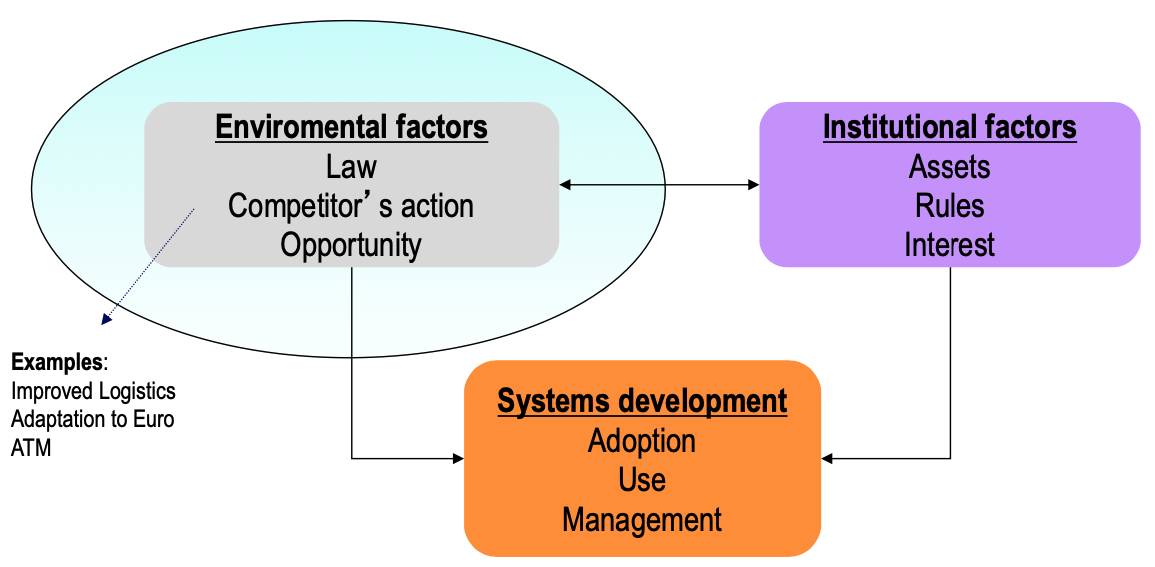
\includegraphics[width=0.7\textwidth]{fotos/2.png}
\caption{Ejemplo de las tareas en el procesamiento de lenguaje natural.}
\label{fig:3.1}
\end{figure}

En la figura \ref{fig:3.1}, se muestra lo que implica entender una oración muy simple en inglés: \textit{A dog is chansing a boy on the playground}. El análisis léxico en este caso implica determinar las categorías sintácticas (partes del discurso) de todas las palabras (por ejemplo, ``\textit{dog}'' es un sustantivo y ``\textit{chasing}'' es un verbo). El análisis sintáctico consiste en determinar que ``\textit{a}'' y ``\textit{boy}'' forman una frase nominal. Lo mismo ocurre con ``\textit{the}'' y ``\textit{playground}'', y ``\textit{on the playground}'' es una frase preposicional. El análisis semántico consiste en mapear las frases nominales a entidades y las frases verbales a relaciones para obtener una representación formal del significado de la oración. Por ejemplo, la frase nominal ``\textit{a boy}'' puede mapearse a una entidad semántica que denota a un niño (es decir, b1), y ``\textit{a dog}'' a una entidad que denota a un perro (es decir, d1). La frase verbal puede mapearse a un predicado de relación ``\textit{chasing}(d1, b1, p1)'' como se muestra en la figura. Nótese que con este nivel de comprensión, también se puede inferir información adicional basada en cualquier conocimiento de sentido común relevante. Por ejemplo, si se asume que si alguien está siendo perseguido puede estar asustado, se podría inferir que el niño que está siendo perseguido (b1) puede estar asustado. Finalmente, el análisis pragmático podría revelar además que la persona que dijo esta oración podría tener la intención de solicitar una acción, como recordar al dueño del perro que vigile al perro. 

\subsection{Desafíos y ambigüedades}

Si bien es posible derivar una representación semántica clara para una oración simple como la que se muestra en la figura \ref{fig:3.1}, en general es muy cimplicado hacer este tipo de análisis para texto en lenguaje natural no restringido. La razón principal de esta dificultad es que el lenguaje natural está diseñado para hacer la comunicación humana eficiente; esto contrasta con un lenguaje de programación, que está diseñado para facilitar la comprensión por parte del ordenador. Específicamente, hay dos razones por las cuales el NLP es muy difícil. 
\begin{itemize}
    \item Se omite mucho conocimiento de sentido común en la comunicación en lenguaje natural porque se asumie que el receptor posee dicho conocimiento (por lo tanto, no hay necesidad de comunicarlo explícitamente).
    \item Se mantienen muchas ambigüedades, que se asumen que el receptor sabe cómo resolver (por lo tanto, no hay necesidad de gastar palabras para aclararlas). Como resultado, el texto en lenguaje natural está lleno de ambigüedad, y resolverla generalmente implicaría razonar con una gran cantidad de conocimiento de sentido común, lo cual es un desafío en inteligencia artificial.
\end{itemize}

En este sentido, el NLP es "completo en IA", es decir, tan difícil como cualquier otro problema complicado en inteligencia artificial.Algunos tipos de ambigüedades a las que hay que enfrentarse en NLP son:
\begin{itemize}
\item Ambigüedad a nivel de palabra: Una palabra puede tener múltiples categorías sintácticas o significados. Por ejemplo, ``diseño'' como sustantivo o verbo, (POS ambiguo) o palabras polisémicas (sentido ambiguo).
\item Ambigüedad sintáctica: Las oraciones pueden tener múltiples estructuras sintácticas. Por ejemplo, procesamiento de lenguaje natural puede tener dos interpretaciones diferentes: ``procesado del lenguaje natural'' o ``procesado natural del lenguaje'' (modificación ambigua). ``Un hombre vio a un niño con un telescopio,'' que tiene interpretaciones diferentes que conducen a significados distintos (adjunción ambigua de frase preposicional (PP)).
\item Resolución de anáforas: Determina a qué se refiere un pronombre, lo cual puede ser poco claro. ``\textit{John persuaded Bill to buy a TB for himself}'', donde ``himself'' puede referirse a John o a Bill.
\item Presuposición: Implica suposiciones, como en ``Él ha dejado de fumar'' implicando que fumaba antes. Hacer este tipo de inferencias resulta generalmente complicado. 
\end{itemize}

\subsection{Historia y estado del arte en NLP}

La investigación en NLP se remonta al menos a la década de 1950, cuando los investigadores eran muy optimistas sobre tener ordenadores capaces de entender el lenguaje humano, particularmente con el propósito de la traducción automática. Sin embargo, pronto quedó claro que la traducción de alta calidad completamente automática no podría lograrse sin conocimiento. Un diccionario resultaba insuficiente; en su lugar, haría falta una enciclopedia. \\

Al darse cuenta de que la traducción automática podría ser demasiado ambiciosa, los investigadores abordaron aplicaciones menos ambiciosas de NLP a finales de la década de 1960 y 1970 con cierto éxito, aunque las técnicas desarrolladas no lograron escalar, teniendo así un impacto limitado en las aplicaciones. Por ejemplo, la gente probó aplicaciones de reconocimiento de voz donde el objetivo es transcribir un discurso. Esta tarea requiere solo una comprensión limitada del lenguaje natural, por lo tanto, es más realista. Se desarrollaron dos proyectos que demostraron la capacidad del ordenador para entender el lenguaje natural: uno es el proyecto Eliza, donde se utilizan reglas superficiales para permitir que un ordenador juegue el papel de un terapeuta para entablar un diálogo en lenguaje natural con un humano; el otro es el proyecto del mundo de bloques, que demostró la viabilidad de la comprensión semántica profunda del lenguaje natural cuando el lenguaje se limita a un dominio de juguete con solo bloques como objetos. \\

En las décadas de 1970 y 1980, se prestó atención al procesamiento de datos textuales en lenguaje natural del mundo real, particularmente a la comprensión de historias. Se desarrollaron muchos formalismos para la representación del conocimiento y reglas heurísticas de inferencia. Sin embargo, la conclusión general fue que incluso las historias simples son bastante difíciles de entender por un ordenador, confirmando la necesidad de una representación del conocimiento a gran escala e inferencias bajo incertidumbre. \\

Después de la década de 1980, los investigadores comenzaron a alejarse de los enfoques simbólicos tradicionales (basados en lógica) para el procesamiento del lenguaje natural, que en su mayoría habían demostrado no ser robustos para aplicaciones reales, y prestaron más atención a los enfoques estadísticos, que dieron más éxito; inicialmente en el reconocimiento de voz, y posteriormente en prácticamente el resto de tareas de NLP. A diferencia de los enfoques simbólicos, los enfoques estadísticos tienden a ser más robustos porque dependen menos de reglas generadas por humanos; en su lugar, a menudo aprovechan las regularidades y patrones en los usos empíricos del lenguaje, y se basan únicamente en datos de entrenamiento etiquetados por humanos y en la aplicación de técnicas de aprendizaje automático. \\

Si bien el conocimiento lingüístico siempre es útil, hoy en día, las técnicas de procesamiento del lenguaje natural más avanzadas tienden a depender en gran medida del uso intensivo de técnicas de aprendizaje automático estadístico, con el conocimiento lingüístico jugando solo un papel secundario. Estas técnicas de NLP estadístico son exitosas para algunas de las tareas de NLP. 

\subsection{Procesamiento de lenguaje natural estadístico}

El NLP estadístico se basa en la probabilidad y en la estadística para resolver problemas de lenguaje natural. Algunas tareas comunes son:
\begin{itemize}
\item El etiquetado de partes del discurso (POS) es una tarea relativamente fácil, y los etiquetadores de POS en el estado del arte pueden tener una precisión muy alta (por encima del 97\% en datos de noticias).
\item El análisis sintáctico (\textit{parsing}) es más difícil, aunque el análisis sintáctico parcial se puede hacer con una precisión razonablemente alta (por ejemplo, por encima del 90\% para el reconocimiento de frases nominales).
\begin{figure}[H]
\centering
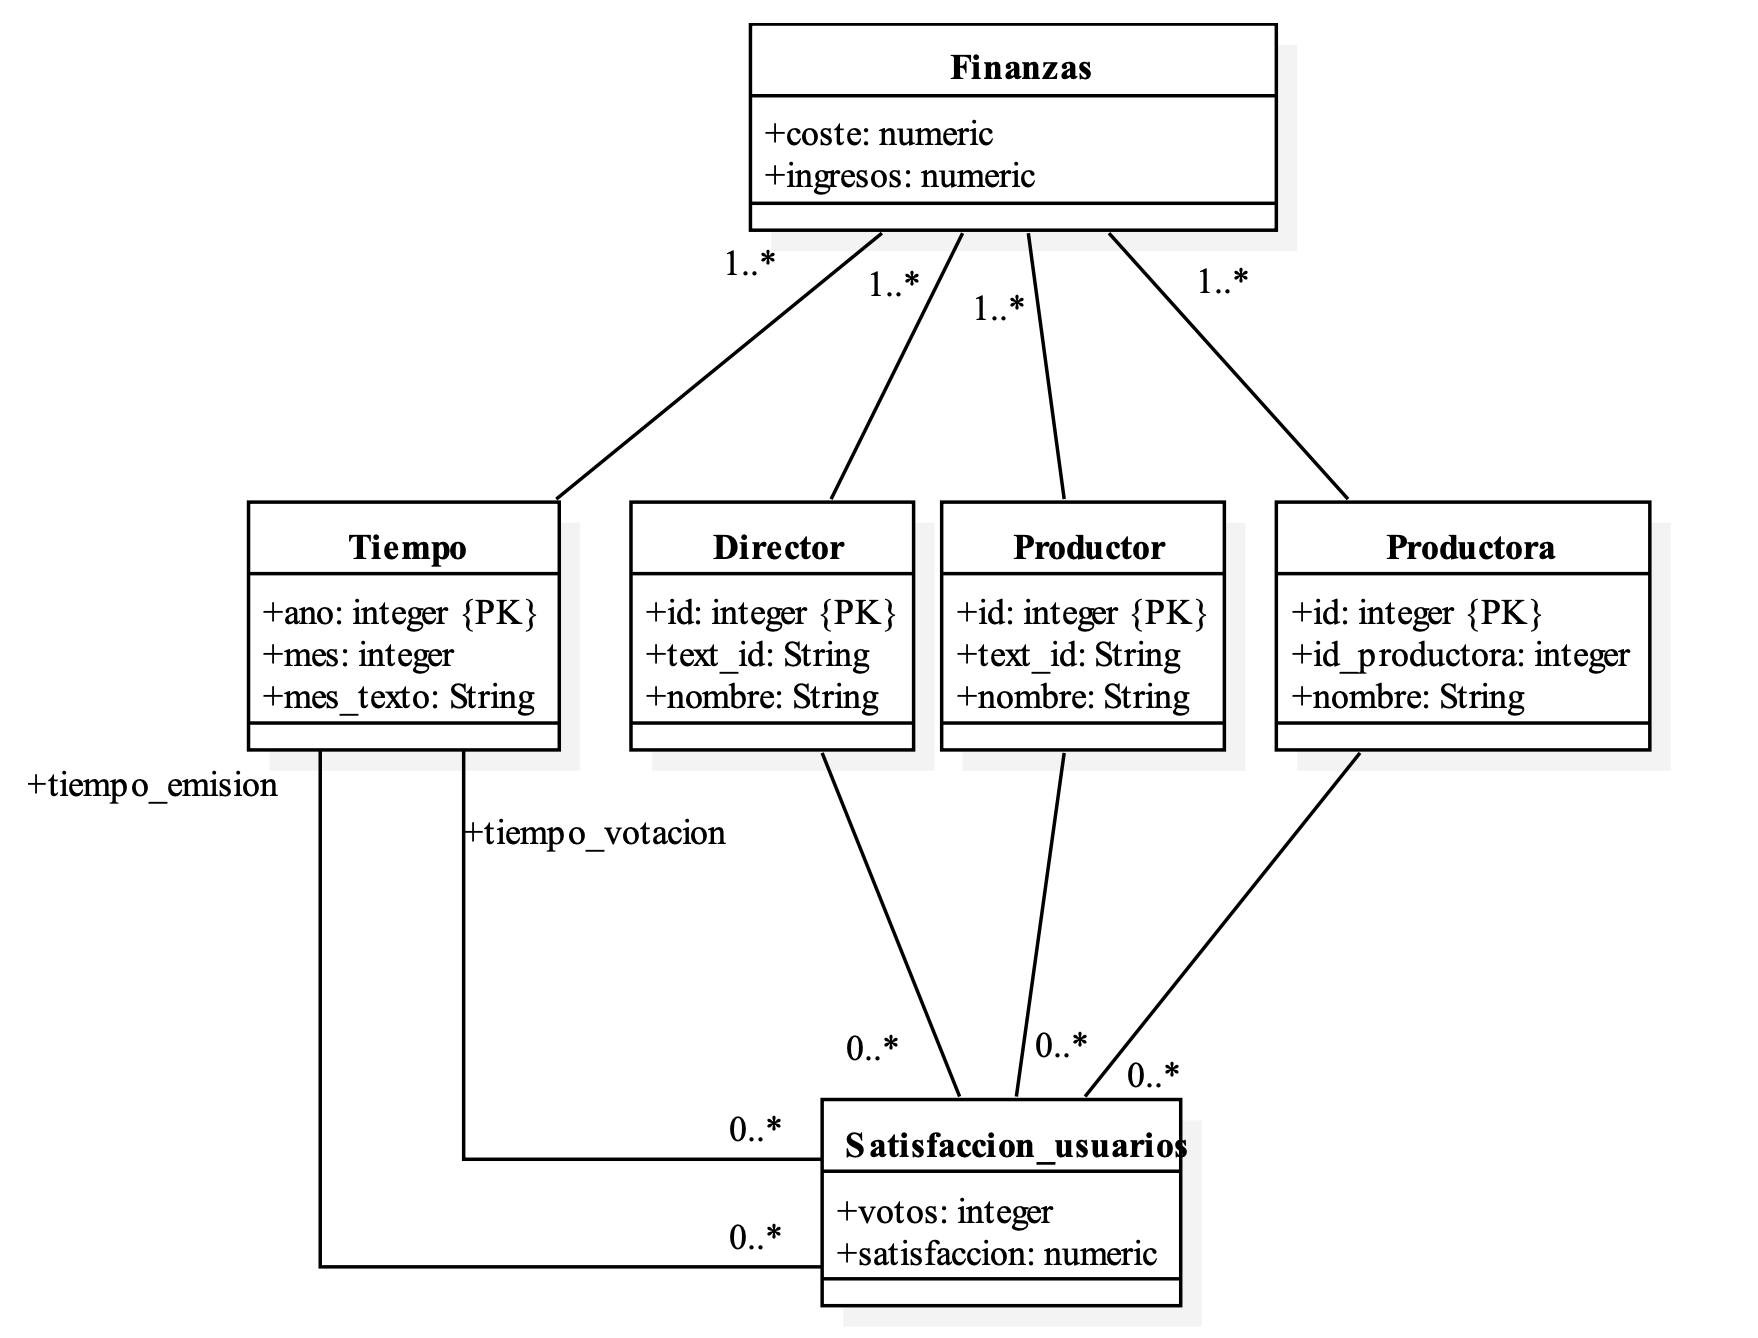
\includegraphics[width=0.25\textwidth]{fotos/3.png}
\caption{Ejemplo de análisis sintáctico.}
\label{fig:3}
\end{figure}
\item Análisis completo de estructura (\textit{full structure parsing}): es una tarea muy complicada debido a las ambigüedades en el lenguaje natural.
\item Análisis semántico: asigna un significado a una oración. Es una tarea aún más complicada, con éxito limitado. Extracción de información notable(se reconocen entidades nombradas como nombres de personas y organizaciones, y relaciones entre entidades como quién trabaja en qué organización), la desambiguación del sentido de las palabras (distinguir diferentes sentidos de una palabra en diferentes contextos de uso) y el análisis de sentimientos (reconocer opiniones positivas sobre un producto en una reseña de producto) son áreas de interés. Inferencias y habla.
\item Análisis de actos: determina la intención detrás de la comunicación. Generalmente, solo es factible en dominios muy limitados.
\end{itemize}

\subsubsection{Procesamiento de lenguaje natural superficial y profundo}   

En textos arbitrarios, solo el análisis superficial del lenguaje natural se puede hacer de forma robusta. El análisis profundo no escala bien, y no es robusto para textos no restringidos. Este último, además, requiere una cantidad significativa de datos de entrenamiento (etiquetados por humanos) para obtener una precisión razonable.

\begin{figure}[h]
\centering
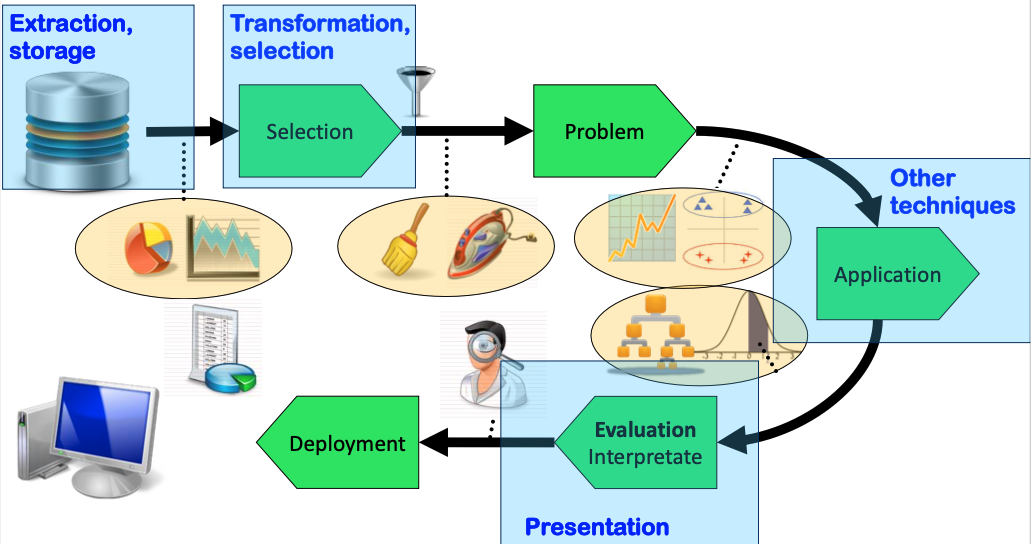
\includegraphics[width=0.5\textwidth]{fotos/4.png}
\caption{Dificultad de varias aplicaciones de NLP.}
\label{fig:4}
\end{figure}

\section{Representación de texto}

Las técnicas de NLP permiten diseñar muchos tipos diferentes de características informativas para los objetos textuales. Como ejemplo, la oración \textit{A dog is chasing a boy on the playground} en la figura \ref{fig:3.3}. Se puede representar esta oración de muchas formas distintas. Primero, siempre se puede representar dicha oración como una cadena de caracteres. Esto es cierto para todos los idiomas, y es quizás la forma más general de representar texto, ya que siempre puede usarse este enfoque para representar cualquier dato textual. Desafortunadamente, la desventaja de esta representación es que no permite realizar análisis semántico, que a menudo es necesario en muchas aplicaciones de minería de texto. No se están reconociendo palabras, que son la unidad básica de significado para cualquier idioma. \\

La siguiente versión de la representación del texto es realizar la segmentación de palabras para obtener una secuencia de palabras. En la oración de ejemplo, se obtienen características como ``\textit{dog}'' y ``\textit{chasing}''. Con este nivel de representación se tiene mucha más libertad. Al identificar palabras, se puede, por ejemplo, descubrir fácilmente las palabras más frecuentes en un documento o en toda la colección. Estas palabras luego se pueden usar para formar temas. Por lo tanto, representar datos textuales como una secuencia de palabras abre muchas posibilidades de análisis interesantes. \\

Sin embargo, este nivel de representación es ligeramente menos general que una cadena de caracteres. En algunos idiomas, como el chino, no es tan fácil identificar todos los límites de las palabras. Para resolver este problema, se confia en algunas técnicas especiales para identificar palabras y realizar una segmentación más avanzada que no se base solo en los espacios en blanco (lo que no siempre es 100\% preciso). Por lo tanto, la representación de la secuencia de palabras no es tan robusta como la representación de la cadena de caracteres. En inglés, es muy fácil obtener este nivel de representación, por lo que puede usarse todo el tiempo. \\

Avanzando más en el procesamiento del lenguaje natural, podemos agregar etiquetas de partes del discurso (POS) a las palabras. Esto permite contar, por ejemplo, los sustantivos más frecuentes, o determinar qué tipo de sustantivos están asociados con qué tipo de verbos. Esto abre más oportunidades para un análisis más profundo. Nótese en la figura \ref{fig:3.3} se usa un signo más en las características adicionales porque al representar el texto como una secuencia de etiquetas de partes del discurso, no necesariamente se reemplaza la secuencia de palabras original. En su lugar, se agrega esto como una forma adicional de representar datos textuales. \\

Representar el texto tanto como palabras como etiquetas de POS enriquece la representación de los datos textuales, permitiendo un análisis más profundo y fundamentado. Si se avanza más, entonces se estaría analizando la oración para obtener una estructura sintáctica. Esto abre más análisis de, por ejemplo, los estilos de escritura o la corrección de errores gramaticales. \\

Avanzando más en el análisis semántico, se podría reconocer ``\textit{dog}'' como un animal. También podemos reconocer ``\textit{boy}'' como una persona, y ``\textit{playground}'' como una ubicación y analizar sus relaciones. Una deducción podría ser que el perro estaba persiguiendo al niño, y el niño está en el parque. Esto agregará más entidades y relaciones, a través del reconocimiento de relaciones entre entidades. Ahora, se puede contar la persona más frecuente que aparece en toda esta colección de artículos de noticias. Estos tipos de patrones repetidos pueden potencialmente dar muy buenas características. \\

Esta representación de alto nivel es aún menos robusta que la secuencia de palabras o las etiquetas de POS, pero es muy útil. No siempre es fácil identificar todas las entidades con los tipos correctos y se pueden cometer errores. Las relaciones son aún más difíciles de encontrar. Si se mueve hacia una representación lógica, entonces existen predicados y reglas de inferencia. Con reglas de inferencia se pueden inferir hechos derivados interesantes del texto. No se puede hacer eso todo el tiempo para todo tipo de oraciones, ya que puede llevar un tiempo de computación significativo o una gran cantidad de datos de entrenamiento. \\

Finalmente, los actos de habla agregarían otro nivel de representación de la intención de esta oración. En este ejemplo, podría ser una solicitud. Saber eso permitiría analizar cosas aún más interesantes sobre el emisor de esta oración. ¿Cuál es la intención de decir eso? ¿Qué escenarios o qué tipos de acciones ocurrirán?

\begin{figure}[h]
\centering
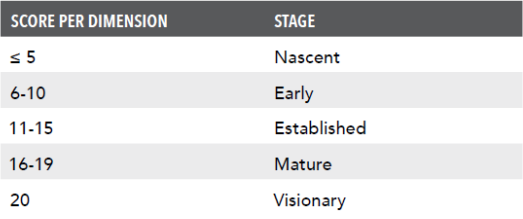
\includegraphics[width=0.7\textwidth]{fotos/5.png}
\caption{Diferentes niveles de representación de texto.}
\label{fig:3.3}
\end{figure}

Las técnicas de NLP más sofisticadas requieren más esfuerzo humano, y generalmente son menos robustas ya que intentan resolver un problema mucho más difícil. Si se analiza el texto en niveles que representan un análisis más profundo del lenguaje, entonces hay que tolerar posibles errores. Eso también significa que aún es necesario combinar dicho análisis profundo con análisis superficial basado en, por ejemplo, secuencias de palabras. A medida que se avanza, la representación del texto está más cerca de la representación del conocimiento en la mente humana; ese es el propósito de la minería de texto. \\

En la representación de textos hay que buscar un balance, un compromiso entre un análisis profundo, que puede dar errores pero dará un conocimiento directo que puede ser extraído del texto, y un análisis superficial, que es robusto pero no aportará una represención del conocimiento con el detalle adecuado. \\

Diferentes representaciones de texto tienden a permitir diferentes análisis, como se muestra en la figura \ref{fig:3.4}. En particular, se agregan gradualmente resultados de análisis más profundos para representar datos textuales que abrirían más oportunidades de representación y capacidades de análisis. 

\begin{figure}[h]
\centering
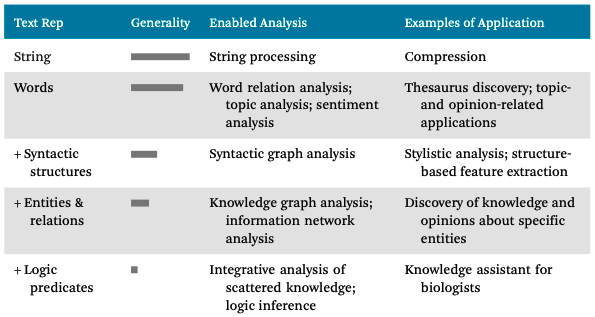
\includegraphics[width=0.7\textwidth]{fotos/8.png}
\caption{Representación de texto y análisis permitido.}
\label{fig:3.4}
\end{figure}

\section{Modelos de lenguaje estadísticos}

Un modelo de lenguaje estadístico proporciona una distribución de probabilidad sobre secuencias de palabras, por ejemplo, 
\begin{align*}
p(\text{\textit{Today is Wednesday}}) &= 0.001 \\
p(\text{\textit{Today Wednesday is}}) &= 0.000000001 \\
p(\text{\textit{The equation has a solution}}) &= 0.000001
\end{align*} 

Un modelo de lenguaje puede depender del contexto. En el modelo de lenguaje mostrado anteriormente, la secuencia ``\textit{The equation has a solution}'' tiene una probabilidad menor que ``\textit{Today is Wednesday}''. Esto puede ser un modelo de lenguaje razonable para describir conversaciones generales, pero puede ser inexacto para describir conversaciones que ocurren en una conferencia de matemáticas, donde la secuencia ``\textit{The equation has a solution}'' puede ocurrir con más frecuencia que ``\textit{Today is Wednesday}''. \\

Sea un modelo de lenguaje, se pueden muestrear secuencias de palabras de acuerdo con la distribución para obtener una muestra de texto. En este sentido, podemos usar dicho modelo para ``generar'' texto. Por lo tanto, un modelo de lenguaje también se denomina a menudo un modelo generativo para texto. 

\subsection{Usos de modelos del lenguaje}

\begin{itemize}
\item Reconocimiento de voz: Predice secuencias probables de palabras. Si se escucha, por ejemplo, \textit{John feels}, se puede predecir que la siguiente palabra será \textit{happy}, aunque haya palabras similares acústicamente, como \textit{habit}. Esto es debido a que una es más probable que la otra. 
\item Categorización de texto: Determina la probabilidad de temas. Por ejemplo, si se tien \textit{baseball} tres vces y \textit{game} una en un artículo, ¿cómo de probable es que el tema sea ``deportes''?
\item Recuperación de información: Mejora la relevancia en búsquedas. Si un usuario está interesado en noticias de deportes, ¿cómo de probable es que se use la palabra \textit{baseball} en una consulta?
\end{itemize}

\subsection{Modelos de lenguaje}

Si se enumeran todas las posibles secuencias de palabras y se asigna una probabilidad a cada secuencia, el modelo sería demasiado complejo de estimar, ya que el número de parámetros es potencialmente infinito al tener un número potencialmente infinito de secuencias de palabras. Es decir, nunca se dispondría de suficientes datos como para estimar estos parámetros. Por lo tanto, se deben hacer suposiciones para simplificar el modelo. \\

El modelo de lenguaje más simple es el modelo de lenguaje unigrama, en el cual se asume que una secuencia de palabras resulta de generar cada palabra de manera independiente. Por lo tanto, la probabilidad de una secuencia de palabras sería igual al producto de la probabilidad de cada palabra. Formalmente, sea $V$ el conjunto de palabras en el vocabulario, y $w_1, \dots, w_n$ una secuencia de palabras, donde $w_i \in V$ es una palabra. Así, la probabilidad de la secuencia de palabras sería
\begin{equation}
p(w_1, \dots, w_n) = \prod_{i=1}^n p(w_i)
\end{equation}

Dado un modelo de lenguaje unigrama $\theta$, habrá tantos parámetros como palabras en el vocabulario, y estos satisfacen la restricción $\sum_{w \in V} p(w) = 1$. Tal modelo esencialmente especifica una distribución multinomial sobre todas las palabras. \\

Dado un modelo de lenguaje $\theta$, en general, las probabilidades de generar dos documentos diferentes $D_1$ y $D_2$ serían diferentes, es decir, $p(D_1 | \theta) \neq p(D_2 | \theta)$. Intuitivamente, los documentos con mayor probabilidad serían aquellos que contienen muchas ocurrencias de las palabras de alta probabilidad según $p(w | \theta)$. En este sentido, las palabras de alta probabilidad de $\theta$ pueden indicar el tema capturado por $\theta$. \\

\begin{figure}[h]
\centering
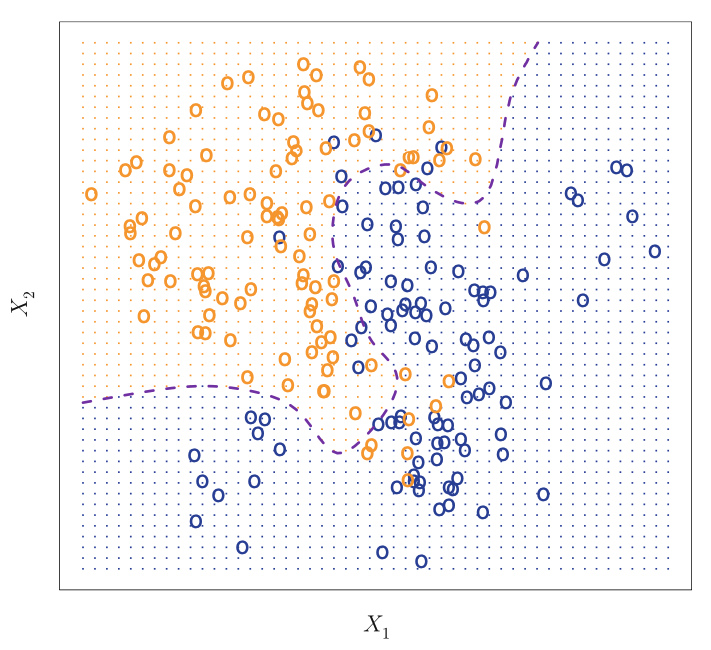
\includegraphics[width=0.4\textwidth]{fotos/9.png}
\caption{Dos ejemplos de modelos de lenguaje unigrama, representando dos temas distintos.}
\label{fig:9}
\end{figure}

Por ejemplo, los dos modelos de lenguaje unigrama ilustrados en la Figura \ref{fig:9} sugieren un tema sobre ``minería de texto'' y un tema sobre ``salud'', respectivamente. Intuitivamente, si $D$ es un artículo sobre minería de texto, se esperaría que $p(D | \theta_1) > p(D | \theta_2)$, mientras que si $D'$ es un artículo de blog que discute el control de la dieta, se esperaría lo contrario: $p(D' | \theta_1) < p(D' | \theta_2)$. También se puede esperar que $p(D | \theta_1) > p(D' | \theta_1)$ y $p(D | \theta_2) < p(D' | \theta_2)$. \\

Sea ahora un documento $D$ que se asume que ha sido generado utilizando un modelo de lenguaje unigrama $\theta$, y se quiere inferir el modelo subyacente $\theta$ (es decir, estimar las probabilidades de cada palabra $w$, $p(w | \theta)$) basado en el documento observado $D$. Este es un problema estándar en estadística llamado estimación de parámetros y puede resolverse utilizando muchos métodos diferentes. \\

Un método popular es el estimador de máxima verosimilitud (ML), que busca un modelo $\hat{\theta}$ que daría a los datos observados la mayor verosimilitud (es decir, que mejor explique los datos):
\begin{equation}
\hat{\theta} = \text{arg max}_{\theta} p(D | \theta)
\end{equation}

Es fácil demostrar que la estimación ML de un modelo de lenguaje unigrama da a cada palabra una probabilidad igual a su frecuencia relativa en $D$. Esto es,
\begin{equation}
p(w | \hat{\theta}) = \frac{\text{c}(w, D)}{|D|}
\end{equation}

donde $c(w, D)$ es el conteo de la palabra $w$ en $D$ y $|D|$ es la longitud de $D$, o el número total de palabras en $D$. \\

Esta estimación es óptima en el sentido de que maximizaría la probabilidad de los datos observados, pero si realmente es adecuada para una aplicación sigue siendo cuestionable. Por ejemplo, si el objetivo es estimar el modelo de lenguaje en la mente de un autor de un artículo de investigación, y usamos el estimador de máxima verosimilitud para estimar el modelo basado solo en el resumen de un artículo, entonces claramente no es correcto, ya que el modelo estimado asignaría una probabilidad cero a cualquier palabra no vista en el resumen, lo que haría que todo el artículo tuviera una probabilidad cero a menos que solo use palabras del resumen. En general, la estimación de máxima verosimilitud asignaría una probabilidad cero a cualquier \textit{token} o evento no observado en los datos; esto es así porque asignar una probabilidad no nula a dicho \textit{token} quitaría masa de probabilidad que podría haberse asignado a una palabra observada (ya que todas las probabilidades deben sumar 1), reduciendo así la verosimilitud de los datos observados. Para mejorar el estimador de máxima verosimilitud se usan técnicas de suavizado. \\

\begin{figure}[h]
\centering
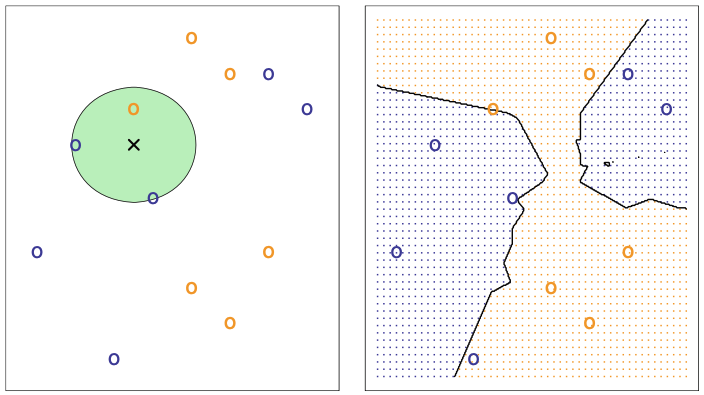
\includegraphics[width=0.7\textwidth]{fotos/10.png}
\caption{Tres modelos de lenguaje diferentes representando tres temas distintos.}
\label{fig:3.6}
\end{figure}

Aunque extremadamente simple, un modelo de lenguaje unigrama es muy útil para el análisis de texto. Por ejemplo, la figura \ref{fig:3.6} muestra tres modelos de lenguaje unigrama diferentes, estimados en tres muestras distintas de datos textuales: una base de datos de texto en inglés general, una base de datos de artículos de investigación en ciencias de la computación y un artículo de investigación sobre minería de texto. En general, las palabras con las probabilidades más altas en los tres modelos son aquellas palabras funcionales en inglés, porque tales palabras se usan frecuentemente en cualquier texto. Bajando más en la lista de palabras, se verían más palabras con contenido y palabras temáticas. Las palabras de contenido serán completamente distintas dependiendo de los datos utilizados para la estimación y, por lo tanto, pueden usarse para discriminar los temas en diferentes muestras de texto. \\

Los modelos de lenguaje unigrama también pueden usarse para realizar análisis semántico de relaciones entre palabras. Por ejemplo, se pueden usarlos para encontrar qué palabras están asociadas semánticamente con una palabra como ``computadora''. La idea principal para hacer esto es ver qué otras palabras tienden a co-ocurrir con esa palabra. Específicamente, primero se puede obtener una muestra de documentos (u oraciones) donde se menciona ``computadora''. Luego se estima un modelo de lenguaje basado en esta muestra para obtener $p(w | \text{computadora})$. Este modelo dice qué palabras ocurren frecuentemente en el contexto de ``computadora''. Sin embargo, las palabras más frecuentes según este modelo probablemente serían palabras funcionales en inglés o palabras que simplemente son comunes en los datos, sin una fuerte asociación con "computadora". Para filtrar las palabras comunes, se necesita un modelo para las mismas, que luego indique qué palabras deben ser filtradas. \\

Es fácil ver que el modelo de lenguaje inglés general (es decir, un modelo de lenguaje de fondo) serviría bien para el propósito. Se puede usar el modelo de lenguaje de fondo para normalizar el modelo $p(w | \text{computadora})$ y obtener una razón, un \textit{ratio} de probabilidad para cada palabra. Las palabras con valores de razón altos pueden entonces asumirse como asociadas semánticamente con ``computadora'', ya que tienden a ocurrir frecuentemente en su contexto, pero no en general. Esto se ilustra en la figura \ref{fig:3.7}.

\begin{figure}[h]
\centering
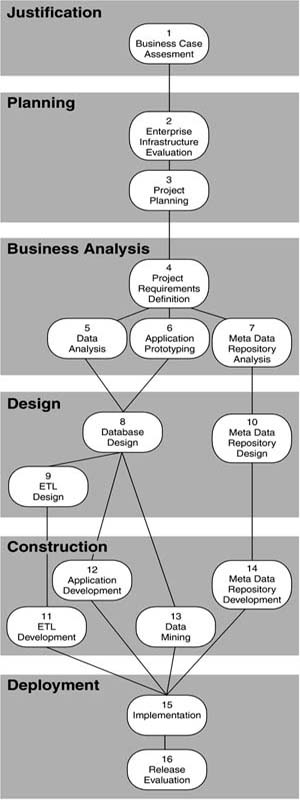
\includegraphics[width=0.7\textwidth]{fotos/11.png}
\caption{Uso de modelos de lenguaje temáticos y modelos de fondo para encontrar palabras semánticamente relacionada.}
\label{fig:3.7}
\end{figure}
\chapter{Cluster Hadoop}\label{ChapterCH} 
% chktex-file 8
% chktex-file 12
% chktex-file 13
% chktex-file 44


\begin{lstlisting}[style=terminal]
    ssh -i "hadoop.pem" ubuntu@DNS_publico_NNRM
    ssh -i "hadoop.pem" -fNT -L 9870:localhost:9870 -L 8088:localhost:8088 ubuntu@DNS_publico_NNRM
    ssh -i "hadoop.pem" -fNT -L 8188:localhost:8188 ubuntu@DNS_publico_BKTL
    yarn --daemon start timelineserver #en BKTL
\end{lstlisting}


echo "ip-172-31-13-193.ec2.internal" >> /opt/bd/hadoop/etc/hadoop/dfs.include
echo "ip-172-31-10-249.ec2.internal" >> /opt/bd/hadoop/etc/hadoop/dfs.include
echo "ip-172-31-6-138.ec2.internal" >> /opt/bd/hadoop/etc/hadoop/dfs.include
echo "ip-172-31-1-58.ec2.internal" >> /opt/bd/hadoop/etc/hadoop/dfs.include ESTE fuera

echo "ip-172-31-1-58.ec2.internal" >> /opt/bd/hadoop/etc/hadoop/dfs.exclude
echo "ip-172-31-1-58.ec2.internal" >> /opt/bd/hadoop/etc/hadoop/yarn.exclude


Nuevos:
echo "ip-172-31-4-16.ec2.internal" >> /opt/bd/hadoop/etc/hadoop/dfs.include
echo "ip-172-31-4-16.ec2.internal" >> /opt/bd/hadoop/etc/hadoop/yarn.include
echo "ip-172-31-0-239.ec2.internal" >> /opt/bd/hadoop/etc/hadoop/dfs.include
echo "ip-172-31-0-239.ec2.internal" >> /opt/bd/hadoop/etc/hadoop/yarn.include


172.31.13.193     /rack1
172.31.10.249     /rack1
172.31.6.138     /rack2
172.31.0.239     /rack3
172.31.4.16     /rack3


TAREA 2:
Cuestion 1: Caben 3: estamos indicando que solo se pueden crear hasta 4 entradas de tipo archivo o directorio en esa ubicación (INCLUYENDO EL PROPIO DIRECTORIO). Al alcanzar la cuota de 4 archivos, el NameNode interrumpe cualquier operación que genere nuevas entradas en ese directorio. Equilibra el uso de recursos del sistema.

Cuestion 2: 

193 - 32 bloques (rack1); 16 - 8 bloques (rack3).

Aparecen 35 bloques under-replicated, 2 perdidos y 1 archivo corrupto. Bloques perdidos 
14. BP-1359368873-172.31.14.95-1729179225409:blk_1073741854_1030 len=67108864 MISSING!
15. BP-1359368873-172.31.14.95-1729179225409:blk_1073741855_1031 len=41943040 MISSING!
Si hay bloques perdidos no se puede recuperar el fichero, ya que no todos los ficheros estan disponibles.


Nuevo datanode: los tres tienen 35 bloques


CUestion 3:
espacio utilizado menor por eficiencia de EC. 

Los datos se dividen en bloques de datos y distribuye entre los datanodes. Da tolerancia a fallos y usa menos espacio.




%----------------------------------------------------------------------------------------
%	BIBLIOGRAPHY
%----------------------------------------------------------------------------------------

\printbibliography[heading=bibintoc, title=References]

%----------------------------------------------------------------------------------------

\end{document}  